%Created by Fredrik Nilsson - freni169 with additions by Johan Billman - johbi142
\documentclass[12pt,a4paper]{article}
\usepackage[utf8]{inputenc}
\usepackage{alltt}
\usepackage[T1]{fontenc}
\usepackage[swedish]{babel}
\usepackage{mathtools}
\usepackage{lmodern}
\usepackage{units}
\usepackage{icomma}
\usepackage{color}
\usepackage{graphicx}
\usepackage{bbm}
\usepackage{tabularx}
\newcommand{\N}{\ensuremath{\mathbbm{N}}}
\newcommand{\Z}{\ensuremath{\mathbbm{Z}}}
\newcommand{\Q}{\ensuremath{\mathbbm{Q}}}
\newcommand{\R}{\ensuremath{\mathbbm{R}}}
\newcommand{\C}{\ensuremath{\mathbbm{C}}}
\newcommand{\rd}{\ensuremath{\mathrm{d}}}
\newcommand{\id}{\ensuremath{\,\rd}}
\usepackage{hyperref}
\usepackage[noindentafter]{titlesec}
\usepackage{color}
\usepackage{mathtools}
\usepackage{float}

\DeclareGraphicsExtensions{.pdf,.png,.jpg}
\DeclarePairedDelimiter\abs{\lvert}{\rvert}%
\DeclarePairedDelimiter\norm{\lVert}{\rVert}%

% Swap the definition of \abs* and \norm*, so that \abs
% and \norm resizes the size of the brackets, and the 
% starred version does not.
\makeatletter
\let\oldabs\abs
\def\abs{\@ifstar{\oldabs}{\oldabs*}}
%
\let\oldnorm\norm
\def\norm{\@ifstar{\oldnorm}{\oldnorm*}}
\makeatother

\renewcommand{\abstractname}{Sammanfattning}


\setlength\parindent{0pt} %%NOINDENT



\title{TDDC74 -  Projektspecifikation}

\author{\textbf{Projektmedlemmar:}\\
Henrik Österman \small{henos134@student.liu.se}\\
Erik Bäcklund Ekvall \small{eriek286@student.liu.se}\\ 
\bigskip\\ \textbf{Handledare:}\\
Johannes Schmidt {\small johannes.schmidt@liu.se}}

\date{\today}
\begin{document}
\maketitle
\newpage

\tableofcontents
\newpage

\section{Projektplanering}
%\textit{Den här delen skriver ni i samband med första inlämningen}\\

The project is supposed to result in a game-engine made specially for making 2D roleplaying games. 
The focus is on making tools to rapidly produce simple games.

The code will be object-oriented primarily, using multiple inheritance but functional code will also be a part of the project. As an example we intend to write our own scripting language which will be functional.

% Ge en kort inledning till projektet (vad är det för spel, vad går det ut på, ...). Det ska vara kort och koncist men ge en tillräcklig förklaring till vad spelet går ut på.

\subsection{Kort projektbeskrivning}
%\textit{Den här delen skriver ni i samband med första inlämningen}\\

A 2D RPG game engine with tools.
Examples of tools are a scripting language for making dialogue, pre-existing class structure which allows quick and easy creation of new objects etc.

We recommend looking at IceBlink Engine and Final Fantasy 4-6 for examples of the type of engine we will try to achieve.

% Om ni skriver ett spel, ge en lite mer genomgående förklaring av spelet och hur det spelas. Om ni gör ett äventyrsspel, inkludera en historia till spelet. Det är bra om ni har en någorlunda omfattande historia så ni har något att utgå från senare \(mer om detta under ADT nedan\). I andra fall kan ni förklara olika scenarios i spelet eller hur det spelas. Till exempel: \"Brickor trillar ned från över delen av skärmen. Dessa kan roteras och målet är att stapla dessa i nedre delen av skärmen och bilda rader.\". Eventuella regler för spelet är även bra att förklara här (för schack till exempel).

\subsection{Utvecklingsmetodik}
%\textit{Den här delen skriver ni i samband med första inlämningen}\\

We will work separately the majority of the time and later have follow-up meetings. In practice this will result in us working in the same room but separately so we can communicate progress as it happens.
We will use git for revision control. The git repo can be found at www.github.com/zappater/riverengine/.

% Hur tänker ni jobba? Ska ni dela upp hur ni skriver koden? Hur kommunicerar ni? Hur delar ni koden mellan varandra och ser till att den är tillgänglig, även om en projektmedlem är sjuk eller borta (ett vanligt problem som uppstår, därför är det viktigt att ni planerar inför detta tidigt)? Tänker ni versionshantera koden (till exempel med subversion eller git)? Jobba kvällar? Helger? Hur lång tid tror ni projektet kommer kräva (bifoga gärna en ungefärlig timplan om ni kan)?

\subsection{Grov tidplan}
%\textit{Den här delen skriver ni i samband med första inlämningen}\\

We will implement one version of both the graphics engine and game engine every week. By the half time meeting we will be working on version 3. Information about what the versions contain can be in the document 'Version.org'.

% Hur ska tiden fördelas? Vad bör göras först? Försök att hålla det på nivån vad gör vi nu direkt, vad ska vara klart till halvtidsmötet och vad sker efter halvtidsmötet. Tänk på att lägga er plan så att ni kan testa projektet så tidigt som möjligt.

\subsection{Betygsambitioner}
%\textit{Den här delen skriver ni i samband med första inlämningen}\\

We will only attempt to achieve the grade 3 on the project as we both already have a 5 in the course from the exams. This allows us to let other courses take more time if they need to.
However we expect to achieve a 5 on the project if we aren't distracted by other courses.

\section{Konceptskiss}
%\textit{Denna del har ni enbart med i projektspecen, ej i slutinlämningen.}\\

For the developer: A lot of code, more like a library than anything else.

For the player: A lot like Final Fantasy, look at the picture and use your imagination.
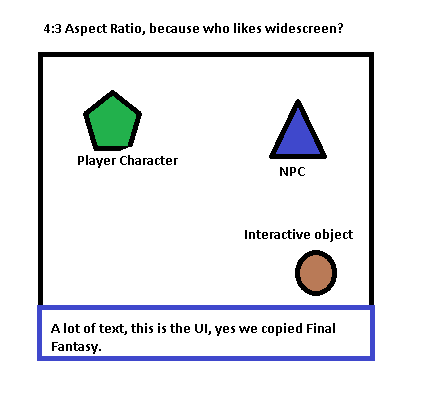
\includegraphics{Koncept_sketch}


% Ge en skiss över tänkt utdata. Gör ni ett grafiskt spel eller program, ge en grov (ritad) skiss över hur det kan se ut. Skriver ni ett textbaserat program, ge påhittad data från en exempelkörning.


\section{Användarmanual}
%\textit{Den här delen skriver ni inför slutinlämningen}\\

The final product includes two parts.
A demo game, this is started by running draw.rkt and a map editor, this is started by running act-editor.rkt.
In addition to this it includes a lot of small subsystems which is explained in the comments to the code.

The demo game is played by running draw.rkt. The character is then moved using the arrow keys and the world is interacted with using the spacebar.
If entering a dialogue with a character the number keys 1, 2, 3 and 4 is used for choosing dialogue options.
The current demo game includes a walkable world, one NPC which can be interacted with by standing next to it and looking at it then pressing the spacebar and two teleporters (without textures so they are invisible) which can also be interacted with using the spacebar.

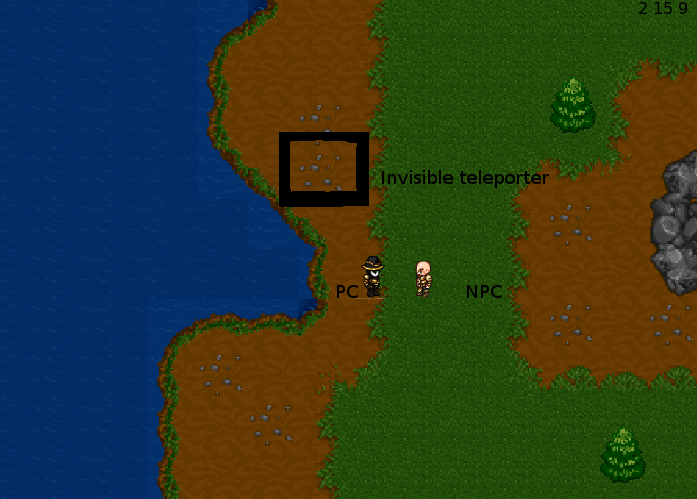
\includegraphics[scale=0.25]{Start}
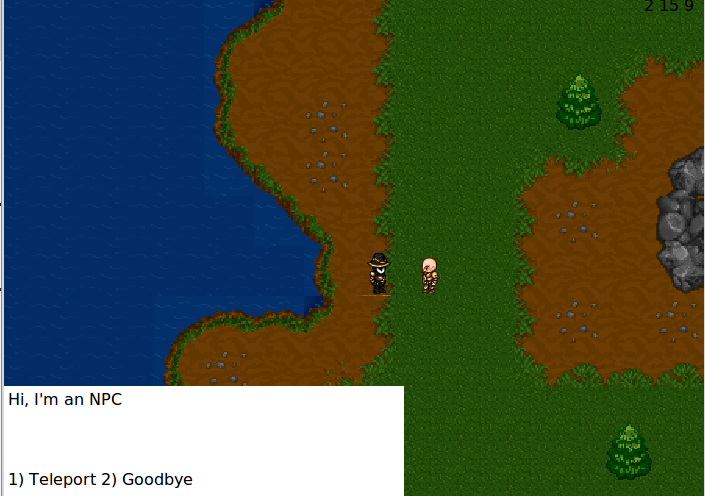
\includegraphics[scale=0.25]{dialogue_with_npc}

The first image shows the start of the game. The second shows conversation with an NPC. And the last image shows where a second teleporter is hidden (you arrive there if you use the first teleporter).

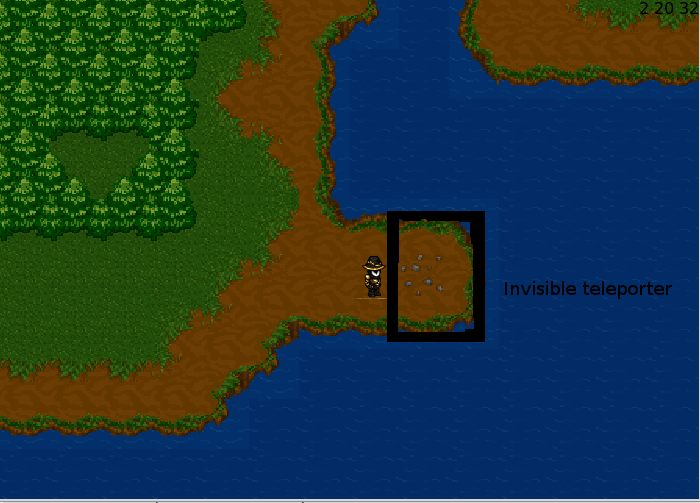
\includegraphics[scale=0.25]{teleporter2}


The map editor is started by running act-editor.rkt. Press h for help and h again to return to the map editor.
Simply put you place tiles using the left mouse button and remove them using the right mouse button.
You scroll through textures using a and q, you change level to put the texture on with s and w.
This will result in a .txt file containing the map. This is then copypasted into a correctly formated .rkt file (make sure to specify language used at the top of the document!). To get a fully running game additional code for objects, required rkt files and control scheme need to be added.
This is a bit too much to explain here, this is after all a game engine not a game maker!
It is made to be a framework for programming your own games within not as a tool for generating complete games without any programming.
We suggest looking at Demo\_game.rkt for an example.


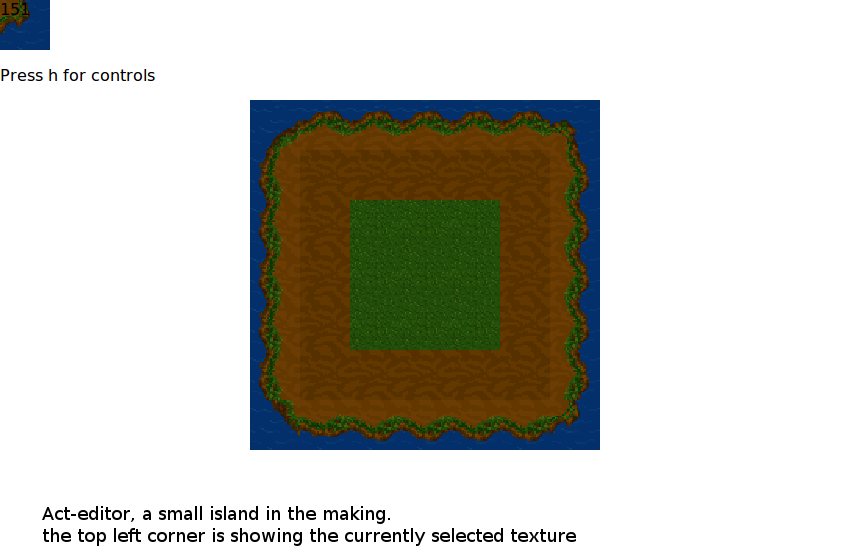
\includegraphics[scale=0.25]{act-editor-example}

%När ni har implementerat ett spel så krävs det en manual som förklarar hur spelet fungerar. Ni ska beskriva spelets olika delar och hur interaktionen fungerar (om mus används, tangentbord, vilka knappar som är aktuella, etc). Inkludera skärmdumpar, som visar hur spelet ser ut. Det ska åtminstone finnas en icke-modifierad bild av spelet. Ett tips i övrigt kan vara att ha en extra bild, ringa in och markera intressanta områden med siffror/färger och beskriva dessa i en prydlig tabell.
%Viktigt: Skriv hur man startar spelet! Vilken fil ska man ladda in och vilken procedur startar man spelet med (om någon sådan)?

\subsection{Kravlista}
%\textit{Den här delen skriver ni i samband med första inlämningen}\\

\bigskip

\begin{tabular}{|c|c|c|}
\hline
\# & \textbf{Beskrivning} & \textbf{Prioritet} \\ \hline
1 & NPC dialogue read from file and scripted using its own language & A \\ \hline
2 & Scripting language for making objects & A \\ \hline
3 & Simple graphic editor & B \\ \hline
4 & 2D graphics engine & A \\ \hline
5 & Scripting language for controlling UI & A \\ \hline
6 & Support for animations & B \\ \hline
\end{tabular}

\bigskip
%även om det finns många triviala ”krav” som kan läggas till (”spelet skall styras med musen”, ...), försök hitta bra krav som återspeglar de karaktäristiska dragen som finns hos ert spel. Eftersom ni under kapitlet ”Arbetsmetodik” har redogjort för önskat betyg, så kan ni genom kraven skapa en övertygelse om att det är just det betyget ni ska ha. Vid osäkerhet kan ni fråga er handledare om råd och tips.

\section{Implementation}
%Det här kapitlet använder ni för att beskriva hur spelet är strukturerat och implementerat. Dels ska ni förklara de abstrakta datatyper ni använder, men även hur dessa används i er kod. Algoritmer och övergripande design passar också in i det här kapitlet (bilder, flödesdiagram, osv. är rekommenderat men ej något krav). Den här delen kan ni strukturera upp enligt egna preferenser. Skapa gärna egna delkapitel för enskilda delar, om det underlättar.

\subsection{Abstrakta datatyper eller klasser}
%\textit{Den här delen skriver ni i samband med första inlämningen och uppdatera inför slutinlämningen}\\

Act: Contains information about what should be read in to memory. It has a type (game or UI). An act contains a n-dimensional vector (in the mathematical meaning) of levels. A game is a collection of acts.


Level: A level is a collection of pointers to objects which are in the same interactionlevel and will be drawn in the same layer by the graphics engine. The difference between interactionlevel and layer is that a interactionlevel determines what the player can interact with while a layer determines when the graphics engine draws the object.


Classes: Items, NPCs, Player Character, World Objects, Sprites, Background. All of these with their own subclasses.

Dialogue will be its own type of ADT. In essence it will be a graph implemented using linked-lists and contained in one or several textfiles. 

%Fundera ut vilka datatyper ni behöver för att implementera spelet. Har ni äventyrsspel och skrivit en bra spelhistoria så har ni vunnit mycket. I princip kan ni bara stryka under substantiv i texten så har ni hittat de flesta datatyperna ni behöver. Beskriv ytterligare hur datatyperna ska kunna användas. Kom ni fram till att ni behöver en stack, så fyller ni på med de procedurer som stacken behöver (till exempel push, pop och size). Hitta ett bra sätt att förklara dessa, gärna tabeller. Det ska vara lättöverskådligt så ni snabbt kan slå upp era procedurer här. Detta kapitel behöver inte vara komplett nu, det viktigaste är att ni börjat tänka på hur ni ska göra. Om ni jobbar mycket med detta kapitel så är det i stort sett bara att sätta igång och koda sen, vilket gör att ni sparar mycket tid. Denna delen fyller ni på ytterligare när ni lämnar in dokumentet igen vid mittavstämningen.

\subsection{Testning}
%\textit{Den här delen skriver ni i samband med första inlämningen}\\

Unit tests will be created as the engine is developed, we are not yet able to specify unit tests.

We will test the system by making a simple techdemo in it. It will contain 1 PC, 2 NPCs with dialogue, 1 interactive world object, 1 item. It will be made in 2 acts.

\subsection{Beskrivning av implementationen}
%\textit{Den här delen skriver ni inför slutinlämningen}\\

For a lot more expansive explanations see the code.
While it is a 2D game engine, the world is built in three dimensions.
A character interacts on a 2D surface called a level, it can only interact with things on its own level.
A level is a mutable datastructure built up as a matrix with each cell containing one object and the coordinates of the cell, if the cell is occupied. An empty cell contains an empty list '() and the coordinates of the cell. 


These levels are then layered on top of each other into a three dimensional datastructure. This is done by placing them into a list (immutable). It is immutable as once a complete world has been built the number of levels should never change while the content in each level may change.
This layering of levels is done in a datastructure called an act, it is essentially a map of the game but as map has other uses in programming I will from now on only use the term act. A map is implemented as an object and functions essentially as the game server. It controls where everything is, it decides where everything is and adds, moves and removes everything from the game world.


A cell can only be occupied by one object at a time. As such this has the interesting implicating that collision detection is automatically implemented. If you want to prevent a character from being able to walk somewhere just place an object in that cell. This is also why the world is constructed as a three dimensional world. If you want to have grass that the character can walk on you need to put the grass on a level lower than that which the character is on. This also allows bridges to be built by for example making a world with four levels. On level one you put a bit of ground, on level two nothing and on level three you put the bridge and on level four nothing.
Now the character will be able to walk under the bridge when on level two and on top of the bridge when on level four. Moving the character between levels is easiest done with the already implemented teleport object, which when used tells the act to move the character to a prespecified place.
I hope this illustrates why the world is constructed as it is.


%Här ska ni förklara hur era datastrukturer och algoritmer fungerar. Det bästa sättet att tänka är lite grann ur någon annan grupps perspektiv. Vad skulle någon annan behöva veta för att förstå en viss del av spelet eller dess implementation? Ni får själva försöka hitta alla dessa delar genom att ställa er själva frågor och studera er kod. Till exempel: "Vad behöver jag veta för att förstå hur rotationsproceduren i mitt Tetris fungerar?".
%Tanken är inte att ni ska skriva och svara på frågor. Detta kan ni snarare se som hjälp för att skriva denna delen. Det finns även ytterligare resurser på kurshemsidan, där ni kan hämta inspiration.

\section{Utvärderingar och erfarenheter}
%\textit{Den här delen skriver ni inför slutinlämningen}\\

%Detta avsnittet är en väldigt viktig del av projektspecifikationen. Här ska ni tänka tillbaka och utvärdera projektet (något som alltid ska göra efter ett projekt). Som en hjälp på vägen kan ni utgå från följande frågeställningar:

Planning the project and datastructure went very well. It works almost exactly as we had imagined with a lot of other benefits which we didn't consider (such as automatic collison detection). What went bad is that we focused on a lot of other courses and did not have the time to implement everything we wanted to. However we still consider the product to be good enough and easy to extend in order to fullfill our original vision.


We probably spent to little time on this project, but at the same time we had a lot of other important things to do. It is hard to say.
The work load was even until the final weeks when implementation of the graphics required a lot more than expected, a part which was primarily on Eriks shoulders.
It is hard to say what should have been done in order to improve the workload balance as the graphics couldn't really be started until the basic datastructure existed and by then a lot of time had already passed by. With a few more weeks of project time the workload would probably have ended up being balanced once again.


The specification has not really been used. What was useful was all the preparation we did before it but we had to do it anyway.
What has been useful is a lot of documentation around the specification such as Versions.org, a document where we in a more flexible way wrote down what, when and how things should be implemented.
We worked as we imagined in the beginning then things broke down towards the end because other courses took up time. When it worked it worked well, when it didn't work things didn't work well.


The hardest problem has been to find time when we are both available and not focused on other courses.
One of the biggest lessons has been to create proper documentation of all code as it is created and take the time to visualize datastructures.
It is much easier to comment and document code while it is being written and if it is already commented it is much easier to change the code.
Ending the project with commenting code for 15h isn't the best thing to do.

Figuring out how to do things when the datastructure is something very abstract can be very hard to do and in the beginning we had to draw our datastructure on a whiteboard several times to understand where we were in it.
Create a lot of help functions if only to make the code easier to understand even if it is something very simple.

%\begin{itemize}
%\item Vad gick bra? Mindre bra?
%\item Lade ni ned för mycket/lite tid?
%\item Var arbetsfördelningen jämn? Om inte: Vad hade ni kunnat göra för att förbättra den?
%\item Har ni haft någon nytta av specifikationen? Vad har varit mest användbart med den? Minst?
%\item Har arbetet fungerat som ni tänkt er? Har ni följt "arbetsmetodiken"? Något som skiljer sig? Till det bättre? Till det sämre?
%\item Vad har varit mest problematiskt, om man utesluter den programmeringstekniska delen? Alltså saker runt omkring, som att hitta ledig tid eller plats att vara på.
%\item Vad har ni lärt er så här långt som kan vara bra att ta med till kommande kurser/projekt?
%\end{itemize}


\section{Tidrapportering}
%\textit{Den här delen skriver ni i samband med första inlämningen och uppdaterar efterhand}\\

Can be found in separate spreadsheet.

%För att veta hur mycket ni har jobbat med projektet, notera antalet timmar och bifoga en timrapport. Börja med detta så fort ni kommit igång med projektspecifikationen! Det är viktigt att ni är ärliga när ni bokför era timmar. Ni lurar bara er själva genom att antingen skriva in mer eller mindre tid, beroende på hur arbetet fortlöpt. Tanken med timrapporteringen är att ni ska få en bättre känsla för hur lång tid en viss uppgift tar att slutföra.
%Eftersom projektet är ganska litet behöver ni inte göra en speciellt omfattande timrapport. Det räcker med att ni för varje vecka noterar hur många timmar som varje gruppmedlem har arbetat. Notera gärna vad för typ av arbetsuppgift som har utförts. Exempelvis kan ni presentera timmarna i en tabell på följande vis:
%\subsection{Person 1}
%\begin{tabular}{|c|c|c|}
%\hline
%Vecka & \textbf{Arbetsuppgift} & \textbf{Tid(h)} \\ \hline
%12 & Skrivit kravspec & 5 \\ \hline
%13 & Implementerat \textit{person}-ADT:n & 2 \\ \hline
%\end{tabular}

%\subsection{Person 2}
%\begin{tabular}{|c|c|c|}
%\hline
%Vecka & \textbf{Arbetsuppgift} & \textbf{Tid(h)} \\ \hline
%12 & Skrivit kravspec & 5 \\ \hline
%13 & Implementerat \textit{person}-ADT:n & 2 \\ \hline
%\end{tabular}
%\\\\
%Se till att ni håller timrapporterna uppdaterade. I samband med mittavstämningen kommer ni skicka in timrapporten till er handledare!


\end{document}
